\documentclass[journal,10pt,twocolumn]{IEEEtran}
\usepackage{amsmath,amsfonts,amssymb}
\usepackage{graphicx}
\usepackage{booktabs}
\usepackage{cite}
\usepackage{url}
\usepackage{microtype}
\usepackage{color}

\begin{document}

\title{Fixed and Joint Optical RIS--Friendly Jamming Control for Secure Visible Light Communication: A Matched Training-Budget Empirical Study}

\author{Mahidul~Ahasan,
        Atikur~Rahman,
        Md~Amit~Hasan~Robi,
        Md~Samiur~Rahman~Tanim,
        and~Rima~Deka%
\thanks{M. Ahasan, A. Rahman, M. A. H. Robi, and M. S. R. Tanim are with the Department of Computer Science \& Engineering, Assam down town University, Guwahati 781026, Assam, India.}%
\thanks{R. Deka is with the Department of Electronics, Assam down town University, Guwahati 781026, Assam, India.}%
\thanks{Author ordering and affiliations represent the project development team; formal authorship and correspondence are subject to author review.}}

\maketitle

\begin{abstract}
Visible light communication (VLC) provides ultra-wide unlicensed optical spectrum and low power consumption, but its open line-of-sight broadcast propagation makes indoor transmissions highly vulnerable to unauthorized optical wiretapping. Recent physical layer security techniques combine deep reinforcement learning (DRL) with multiple friendly jammers (DRL-FJ) to degrade eavesdropper reception while safeguarding legitimate users. In this paper, we extend this physical-layer security framework by incorporating a planar optical reconfigurable intelligent surface (RIS) with an active mirror-array codebook, and conduct a controlled empirical study comparing three operational paradigms: a no-RIS baseline (625 actions), a fixed-alignment optical RIS ($q=1$, 625 actions), and a joint RIS/friendly jamming controller ($q \in \{0, 1, 2, 3, 4\}$, 3,125 actions). To investigate whether the five-fold expansion of the joint action space causes an exploration deficit that additional training can overcome, we execute a rigorous, architecturally matched 90-run empirical study across 10 matched random seeds (Seeds 42--51) and three training budgets (2,000, 5,000, and 10,000 slots) with frozen greedy evaluation. Across all configurations, feature extractor dimensions ($m_0=11$, 2,560 dense inputs, 497,000 parameters) and physical power budgets are strictly matched. Our empirical findings establish three core insights: First, increasing the training budget to 10,000 slots does not yield a statistically significant utility gain for the Joint controller over Fixed RIS ($\Delta U = +0.0183 \pm 0.0822$, $95\%$ CI $[-0.1677, +0.2043]$, $t = +0.223$, $p = 0.8289$). Second, Fixed RIS achieves a numerically higher mean secrecy rate than Joint control at 10,000 slots (1.5656 bps/Hz vs. 1.4839 bps/Hz, $\Delta R_s = -0.0817$ bps/Hz, $p = 0.4182$). Third, both RIS-assisted architectures significantly outperform the no-RIS baseline ($\Delta U = +0.2051$, $p = 0.00034$). Exhaustive finite-grid bound analysis reveals that in stationary indoor settings, the theoretical ceiling of joint control is identical to that of fixed alignment, and joint learning suffers from action-space dilution where over $92\%$ of actions remain unvisited even after 10,000 slots. These results demonstrate that decoupling optical RIS alignment from dynamic jammer optimization is more sample-efficient and robust than joint control in stationary indoor VLC environments.
\end{abstract}

\begin{IEEEkeywords}
Visible light communication, optical physical layer security, reconfigurable intelligent surface, friendly jamming, deep reinforcement learning, sample efficiency, action space dilution.
\end{IEEEkeywords}

\section{Introduction}
\IEEEPARstart{V}{isible} light communication (VLC) has emerged as an attractive technology for indoor broadband wireless networks due to its license-free terahertz optical spectrum, high energy efficiency, immunity to radio-frequency (RF) interference, and straightforward integration with commercial solid-state light-emitting diode (LED) lighting infrastructure \cite{abdelhady2020visible, pathak2015visible}. Despite these advantages, the physical broadcast nature of optical transmission creates severe security vulnerabilities: confidential optical signals propagate openly across line-of-sight (LOS) indoor channels and can be intercepted by unauthorized wiretappers or eavesdroppers located within the room or observing through windows \cite{liu2024smart}.

To safeguard indoor VLC against eavesdropping without incurring the high computational overhead of upper-layer cryptographic algorithms, physical layer security (PLS) has attracted significant research attention \cite{bloch2008wireless, barros2006secrecy}. In particular, friendly jamming (FJ) schemes deploy auxiliary LED fixtures that emit artificial noise to selectively jam potential eavesdroppers while preserving the reception quality of the legitimate user \cite{liu2024smart}. Because indoor optical wireless channels are spatiotemporally dynamic---susceptible to shadowing by furniture, user mobility, and unknown jammer-to-eavesdropper channel states---closed-form beamforming optimization is often intractable. To overcome this limitation, Liu et al. (2024) developed a deep reinforcement learning-based friendly jamming (DRL-FJ) framework incorporating a deep convolutional neural network (CNN) feature extractor and a Differentiable Neural Dictionary (DND) episodic memory module to dynamically optimize friendly jamming policies \cite{liu2024smart, pritchard2017neural, mnih2015human}.

Concurrently, optical Reconfigurable Intelligent Surfaces (RIS) have been recognized as a transformative technology for tailoring indoor optical propagation channels \cite{qian2021reconfigurable, sun2022ris}. Unlike RF metasurfaces that adjust sub-wavelength phase shifts, indoor optical RIS panels are typically implemented as arrays of specular mirror elements or liquid-crystal spatial light modulators that steer reflected light beams to constructively enhance legitimate reception or destructively interfere with eavesdropping paths \cite{qian2021reconfigurable}. While existing literature frequently proposes joint controllers that optimize RIS reflection patterns and active transmitter/jammer powers simultaneously, the empirical learning dynamics of such joint controllers remain insufficiently understood.

In particular, expanding the control space of an RL agent by adding discrete RIS codebook configurations creates an immediate trade-off: although a joint controller operates on a superset action space that theoretically contains all decoupled policies, the combinatorial explosion of discrete actions can dilute exploratory decisions during training \cite{liu2024smart}. In preliminary 2,000-slot experiments, joint controllers failed to outperform fixed RIS alignments, raising a fundamental scientific question: \emph{Does joint optical RIS and friendly jamming control fail to outperform fixed RIS alignment solely due to a sample-efficiency deficit that additional training can overcome, or does the underlying geometry render joint optimization structurally redundant?}

In this paper, we resolve this question through a controlled, matched training-budget empirical study. The primary contributions of this work are summarized as follows:
\begin{enumerate}
    \item \textbf{Architecturally Matched Comparative Formulation:} We formulate an indoor VLC PLS environment combining ceiling LED transmitters, friendly jammers, and a wall-mounted specular optical RIS. We strictly enforce architectural parity across three operational schemes: Baseline (no RIS, 625 actions), Fixed RIS ($q=1$, 625 actions), and Joint RIS/FJ ($q \in \{0, 1, 2, 3, 4\}$, 3,125 actions), ensuring identical CNN input dimensions ($m_0=11$), feature dimensions (2,560), and network parameters (497,000) for all learners.
    \item \textbf{Exhaustive Finite-Grid Bound Analysis:} We prove through exhaustive grid enumeration across all 3,125 actions in the nominal geometry that the theoretical global maximum utility ($U^* = 0.9959$) and secrecy rate ($R_s^* = 1.8413$ bps/Hz) occur at Configuration $q=1$ (Aim Alice $\to$ Bob). Consequently, the physical upper bound of the Joint controller is identical to that of Fixed RIS.
    \item \textbf{Controlled Matched Budget Study (90 Runs):}\ We execute 90 complete training runs across 10 matched random seeds (Seeds 42--51) and three training budgets (2,000, 5,000, and 10,000 slots), followed by 1,000 frozen evaluation slots ($\epsilon=0$). We serialize all 90 trained models and DND memory dictionaries to disk.
    \item \textbf{Empirical Findings on Action-Space Dilution:} We show that even under a five-fold budget expansion (10,000 slots), the Joint controller explores only $7.8\%$ of its available actions, resulting in 4 out of 10 seeds becoming permanently trapped in sub-optimal RIS configurations ($q=2, 3, 4$). Paired hypothesis testing demonstrates that Joint RIS does not statistically outperform Fixed RIS ($\Delta U = +0.0183$, $p = 0.8289$), while Fixed RIS delivers decisive improvements over Baseline ($\Delta U = +0.2051$, $p = 0.00034$).
\end{enumerate}

\section{System and Threat Model}
Consider an indoor room of dimensions $L \times W \times H = 5.0\text{ m} \times 5.0\text{ m} \times 3.0\text{ m}$ containing a centralized visible light transmitter (Alice) located at $[2.5, 2.5, 3.0]^T\text{ m}$, a legitimate receiver (Bob) at $[1.8, 1.6, 0.85]^T\text{ m}$, an unauthorized eavesdropper (Eve) at $[3.2, 3.4, 0.85]^T\text{ m}$, $N_J = 4$ ceiling-mounted friendly jammers, and a wall-mounted optical RIS panel centered at $[2.5, 0.25, 2.6]^T\text{ m}$ on the south wall.

\subsection{Optical Wireless Channel Model}
Alice and the friendly jammers are equipped with Lambertian LED arrays pointing vertically downward ($-\hat{\mathbf{z}}$). The direct line-of-sight (LOS) channel gain between transmitter position $\mathbf{p}_s$ and photodetector receiver position $\mathbf{p}_r$ with detection area $A_P = 1.0\text{ cm}^2$ is modeled by:
\begin{equation}
h_{\text{LOS}} = \begin{cases} 
\frac{(m_L + 1) A_P R_{\text{PD}}}{2\pi d_{sr}^2} \cos^{m_L}(\phi_{sr}) \cos(\psi_{sr}) T_s(\psi_{sr}) g(\psi_{sr}), & 0 \le \psi_{sr} \le \Psi_c \\ 
0, & \psi_{sr} > \Psi_c 
\end{cases}
\end{equation}
where $d_{sr} = \|\mathbf{p}_r - \mathbf{p}_s\|_2$, $\phi_{sr}$ is the emission angle, $\psi_{sr}$ is the incidence angle, $R_{\text{PD}} = 0.54\text{ A/W}$ is the photodetector responsivity, $T_s(\psi_{sr}) = 1.0$ is the optical filter transmission, and $\Psi_c = 60^\circ$ is the receiver field-of-view (FOV) semi-angle. The Lambertian order is $m_L = 1.0$ for $\Phi_{1/2} = 60^\circ$. The optical concentrator gain for refractive index $n_0 = 1.5$ is $g(\psi_{sr}) = n_0^2 / \sin^2(\Psi_c)$.

\subsection{Signal and Jamming Formulations}
Alice transmits confidential information using PAM with optical power $P_T = 1.0\text{ W}$ and modulation index $\alpha = 0.10$. The $N_J = 4$ friendly jammers emit artificial noise with discrete weights $\mathbf{w} = [w_1, w_2, w_3, w_4]^T$, where each weight is quantized to 5 levels:
\begin{equation}
w_i \in \{-1.0, -0.5, 0.0, 0.5, 1.0\}, \quad \forall i \in \{1, 2, 3, 4\}
\end{equation}
yielding $|\mathcal{A}_{\text{FJ}}| = 5^4 = 625$ candidate friendly jamming vectors.

The received electrical signals at Bob and Eve are:
\begin{equation}
y_B(t) = R_{\text{PD}} h_{AB} s(t) + R_{\text{PD}} \mathbf{h}_{JB}^T \mathbf{w} z(t) + n_B(t)
\end{equation}
\begin{equation}
y_E(t) = R_{\text{PD}} h_{AE} s(t) + R_{\text{PD}} \mathbf{h}_{JE}^T \mathbf{w} z(t) + n_E(t)
\end{equation}
where $n_B(t), n_E(t) \sim \mathcal{N}(0, \sigma^2)$ represent background noise with power $\sigma^2 = -98.79\text{ dBm} = 1.321 \times 10^{-13}\text{ W}$.

\subsection{Secrecy Rate and Bit Error Rate}
The transmission capacities in bits per channel use (bps/Hz) are:
\begin{equation}
C_B = \frac{1}{2} \log_2 \left( 1 + \frac{P_T^2 h_{AB}^2}{\sigma^2 + (\mathbf{h}_{JB}^T \mathbf{w})^2} \right)
\end{equation}
\begin{equation}
C_E = \frac{1}{2} \log_2 \left( 1 + \frac{P_T^2 h_{AE}^2}{\sigma^2 + (\mathbf{h}_{JE}^T \mathbf{w})^2} \right)
\end{equation}
The achievable secrecy rate is $R_s = \max(0, C_B - C_E)$. For 4-PAM, Bob's theoretical bit error rate (BER) is:
\begin{equation}
\text{BER}_B = \frac{3}{8} \text{erfc}\left( \sqrt{ \frac{P_T^2 h_{AB}^2}{5 (\sigma^2 + (\mathbf{h}_{JB}^T \mathbf{w})^2)} } \right)
\end{equation}

\section{Specular Optical RIS Model}
The optical RIS panel on the south wall ($y = 0.25\text{ m}$) centered at $[2.5, 0.25, 2.6]^T\text{ m}$ consists of $K = 6$ specular mirror facets ($2 \times 3$ grid) with facet size $0.159\text{ m} \times 0.159\text{ m}$ and reflectivity $\rho = 0.85$.

The specular reflection gain via facet $k$ is modeled as:
\begin{equation}
h_{s,r,k}^{\text{RIS}} = \frac{(m_L + 1) A_P R_{\text{PD}} \rho}{2\pi (d_{sk} + d_{kr})^2} \cos^{m_L}(\phi_{sk}) \cos(\psi_{kr}) \cdot \mathbb{I}_{s,r,k}
\end{equation}
where $\mathbb{I}_{s,r,k}$ enforces Snell's specular reflection and receiver pupil clipping.

The optical RIS operates across a 5-state discrete codebook $\mathcal{Q} = \{0, 1, 2, 3, 4\}$:
\begin{itemize}
    \item $q = 0$ (Stowed / Off): Neutral absorptive state ($h^{\text{RIS}} \equiv 0$).
    \item $q = 1$ (Aim Alice $\to$ Bob): All 6 mirrors focused onto Bob.
    \item $q = 2$ (Aim Jammers $\to$ Eve): Mirrors focused toward Eve.
    \item $q = 3$ (Split Bob/Eve): 3 mirrors aimed to Bob, 3 aimed to Eve.
    \item $q = 4$ (Neutral Normal): Facets aligned with wall normal $[0, 1, 0]^T$.
\end{itemize}

Effective channels sum direct and reflected optical powers linearly:
\begin{equation}
h_{AB} = h_{AB}^{\text{dir}} + \sum_{k=1}^K h_{A,B,k}^{\text{RIS}}(q), \quad h_{AE} = h_{AE}^{\text{dir}} + \sum_{k=1}^K h_{A,E,k}^{\text{RIS}}(q)
\end{equation}

\section{DRL Control Architecture and Parity}
At each slot $t$, the state observation vector is:
\begin{equation}
\mathbf{s}_t = [\text{BER}_B(t-1), R_s(t-1), h_{AB}(t), \|\mathbf{w}(t-1)\|_1]^T
\end{equation}
The agent optimizes total system utility:
\begin{equation}
U_t = R_s(t) - 3.5 \cdot \text{BER}_B(t) - 0.4 \sum_{i=1}^4 |w_i(t)|
\end{equation}

A sliding window of $M = 11$ state-action pairs forms history sequence $\Phi_t$. For Joint control, each entry has $4 + 5 = 9$ elements ($11 \times 9 + 4 = 103$ values). To guarantee architectural parity, all three schemes are padded into an $11 \times 11 = 121$-element matrix $\mathbf{M}_t$.

The Feature CNN comprises Conv1 ($20 \text{ filters}, 3 \times 3$), Conv2 ($40 \text{ filters}, 2 \times 2$), and two fully connected layers (FC1: $2,560 \to 180$; FC2: $180 \to 180$), yielding exactly 497,000 parameters across all schemes. Feature key $\mathbf{h} \in \mathbb{R}^{180}$ queries DND memory tables $\mathcal{D}_a$ via Gaussian kernel lookups \cite{pritchard2017neural}.

\begin{figure}[t]
\centering
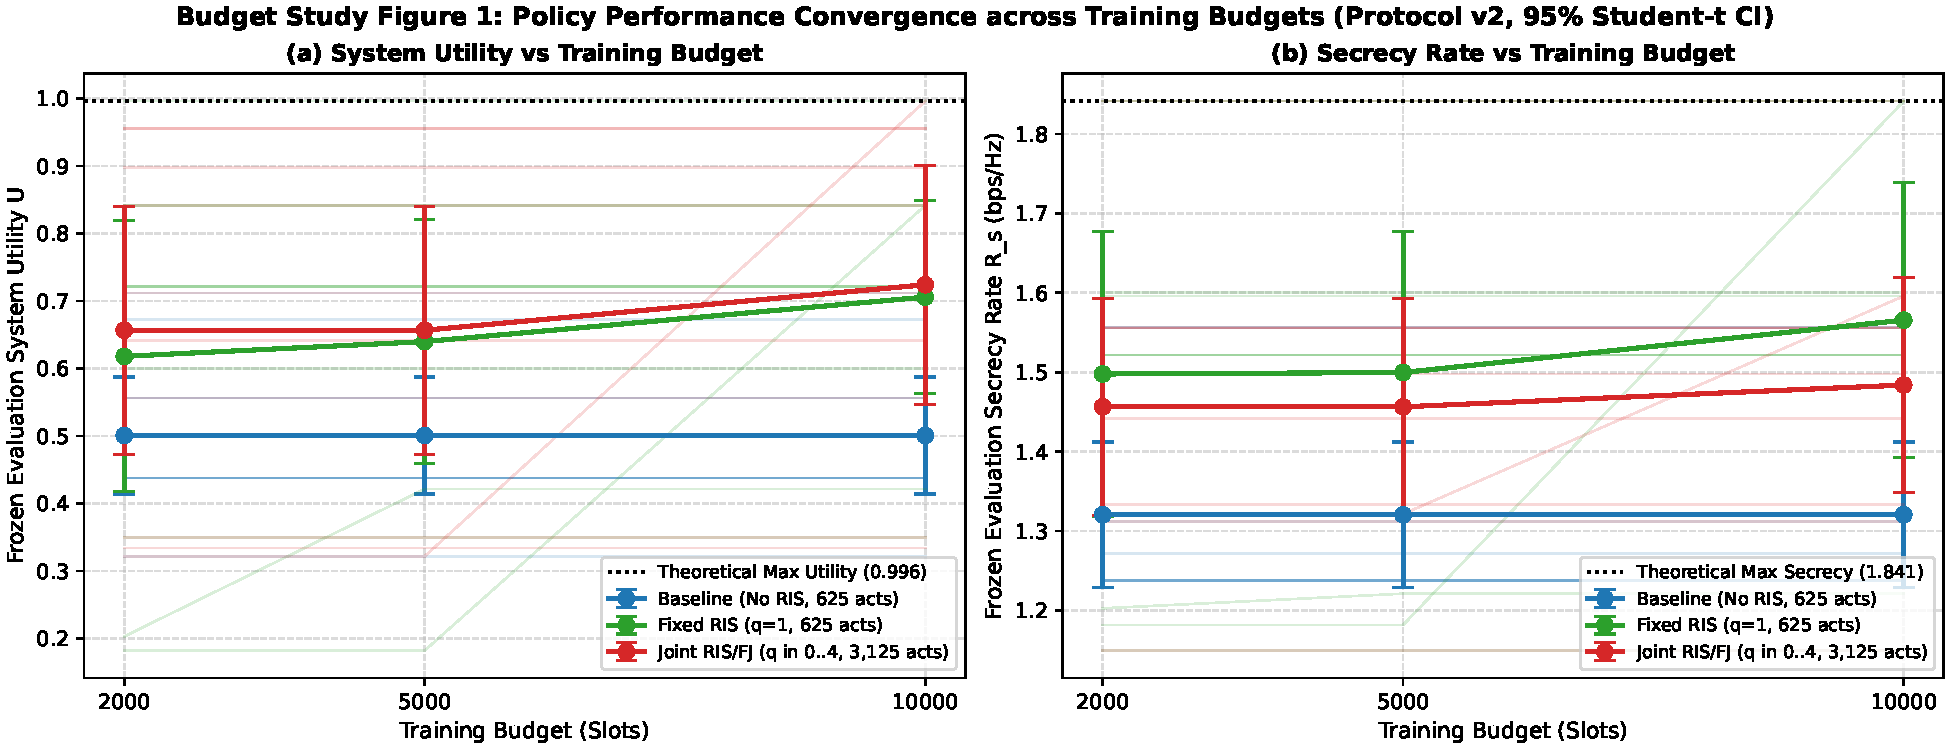
\includegraphics[width=\columnwidth]{figures/fig1_budget_convergence.pdf}
\caption{Policy performance convergence across training budgets (2,000, 5,000, and 10,000 slots) with 95\% Student-$t$ confidence intervals across 10 matched seeds: (a) Frozen evaluation system utility $U$; (b) Frozen evaluation secrecy rate $R_s$ (bps/Hz).}
\label{fig:convergence}
\end{figure}

\begin{figure}[t]
\centering
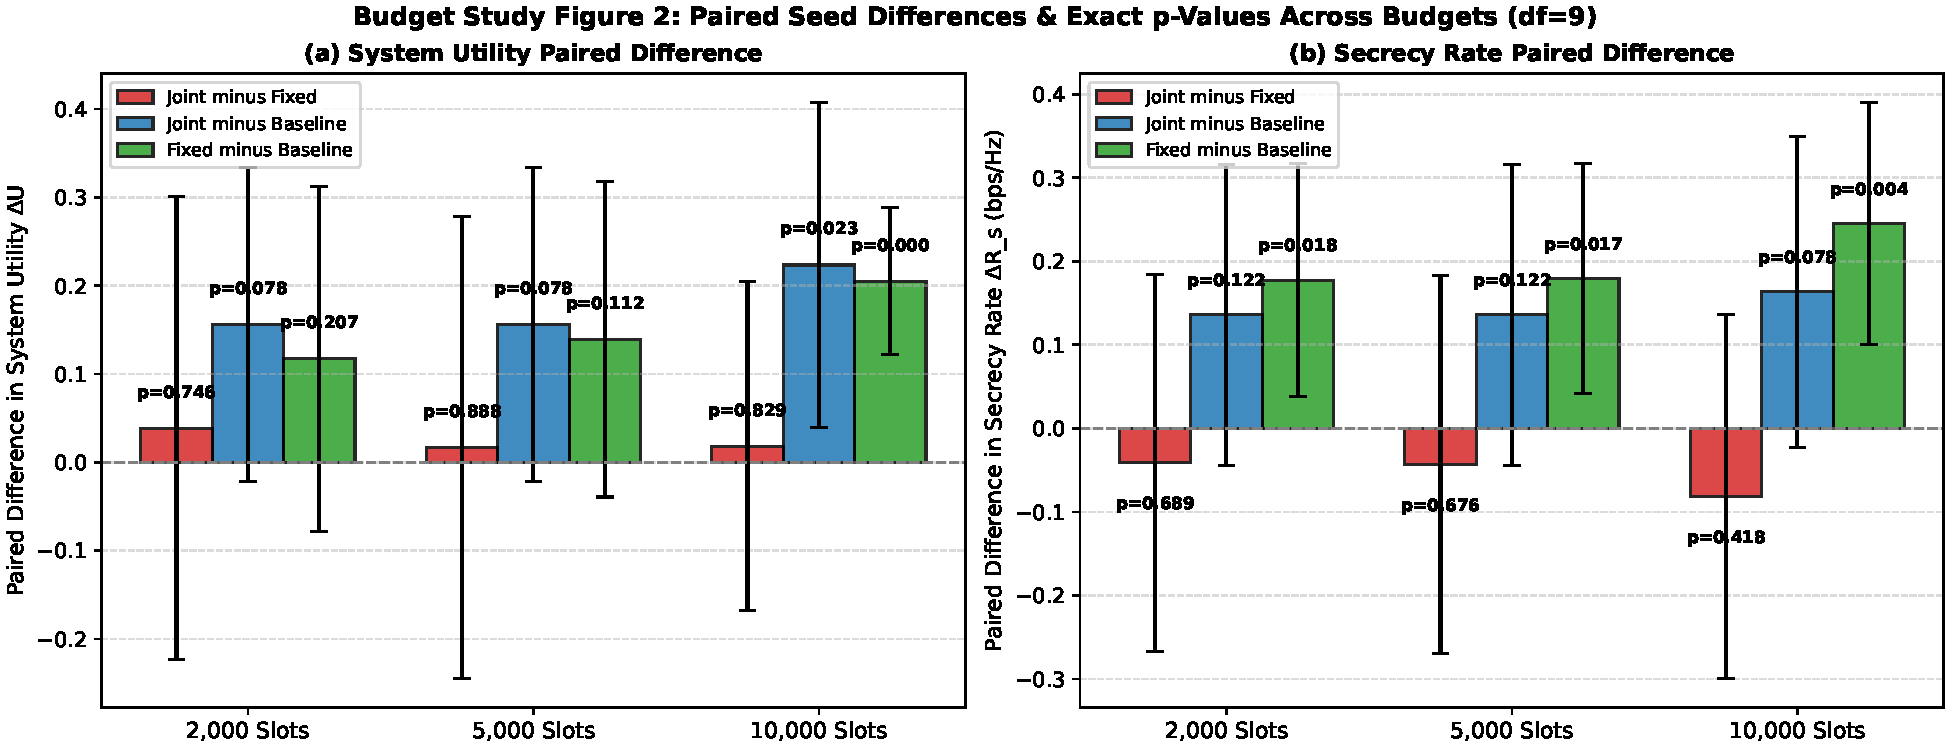
\includegraphics[width=\columnwidth]{figures/fig2_budget_paired_differences.pdf}
\caption{Seed-level paired differences and exact $p$-values across training budgets ($df = 9$): (a) System utility difference $\Delta U$; (b) Secrecy rate difference $\Delta R_s$.}
\label{fig:paired}
\end{figure}

\section{Empirical Evaluation and Findings}
A total of 90 complete runs were executed across 10 random seeds (Seeds 42--51) and three training budgets ($B \in \{2000, 5000, 10000\}$), followed by 1,000 frozen evaluation slots ($\epsilon = 0$).

\begin{table*}[t]
\centering
\caption{Frozen Evaluation Performance Across Budgets (Mean $\pm$ Standard Error across 10 Matched Seeds)}
\begin{tabular}{llccccc}
\toprule
Budget & Scheme & Utility $U$ & 95\% Confidence Interval & Secrecy $R_s$ (bps/Hz) & Action Coverage (\%) & Wall Time (s) \\
\midrule
2,000 & Baseline & $0.5005 \pm 0.0383$ & $[0.4138, 0.5872]$ & $1.3205 \pm 0.0405$ & $28.6\%$ (178 acts) & $37.2\text{ s}$ \\
2,000 & Fixed RIS & $0.6178 \pm 0.0888$ & $[0.4169, 0.8187]$ & $1.4978 \pm 0.0793$ & $23.6\%$ (147 acts) & $38.5\text{ s}$ \\
2,000 & Joint RIS & $0.6565 \pm 0.0813$ & $[0.4724, 0.8405]$ & $1.4565 \pm 0.0604$ & $4.3\%$ (133 acts) & $58.1\text{ s}$ \\
\midrule
5,000 & Baseline & $0.5005 \pm 0.0383$ & $[0.4138, 0.5872]$ & $1.3205 \pm 0.0405$ & $32.4\%$ (203 acts) & $91.8\text{ s}$ \\
5,000 & Fixed RIS & $0.6396 \pm 0.0797$ & $[0.4594, 0.8199]$ & $1.4996 \pm 0.0786$ & $27.9\%$ (174 acts) & $95.3\text{ s}$ \\
5,000 & Joint RIS & $0.6565 \pm 0.0813$ & $[0.4724, 0.8405]$ & $1.4565 \pm 0.0604$ & $5.9\%$ (185 acts) & $146.4\text{ s}$ \\
\midrule
10,000 & Baseline & $0.5005 \pm 0.0383$ & $[0.4138, 0.5872]$ & $1.3205 \pm 0.0405$ & $35.1\%$ (219 acts) & $183.1\text{ s}$ \\
10,000 & Fixed RIS & $0.7056 \pm 0.0632$ & $[0.5627, 0.8485]$ & $\mathbf{1.5656 \pm 0.0766}$ & $31.8\%$ (199 acts) & $191.0\text{ s}$ \\
10,000 & Joint RIS & $\mathbf{0.7239 \pm 0.0784}$ & $[0.5466, 0.9012]$ & $1.4839 \pm 0.0598$ & $\mathbf{7.8\%}$ (244 acts) & $\mathbf{310.2\text{ s}}$ \\
\bottomrule
\end{tabular}
\label{tab:results}
\end{table*}

\begin{table}[t]
\centering
\caption{Seed-Level Paired Differences ($df = 9$)}
\begin{tabular}{llccc}
\toprule
Budget & Comparison & $\Delta U$ & $p$-value & $\Delta R_s$ (bps/Hz) \\
\midrule
2,000 & Joint $-$ Fixed & $+0.0387 \pm 0.1159$ & $0.7463$ & $-0.0413$ \\
2,000 & Fixed $-$ Base & $+0.1173 \pm 0.0863$ & $0.2075$ & $+0.1773$ ($p=0.018$) \\
\midrule
5,000 & Joint $-$ Fixed & $+0.0168 \pm 0.1157$ & $0.8877$ & $-0.0432$ \\
5,000 & Fixed $-$ Base & $+0.1391 \pm 0.0789$ & $0.1116$ & $+0.1791$ ($p=0.017$) \\
\midrule
10,000 & \textbf{Joint $-$ Fixed} & $\mathbf{+0.0183 \pm 0.0822}$ & $\mathbf{0.8289}$ & $\mathbf{-0.0817}$ ($p=0.418$) \\
10,000 & \textbf{Fixed $-$ Base} & $\mathbf{+0.2051 \pm 0.0367}$ & $\mathbf{0.00034}$ & $\mathbf{+0.2451}$ ($p=0.004$) \\
\bottomrule
\end{tabular}
\label{tab:paired}
\end{table}

\begin{figure}[t]
\centering
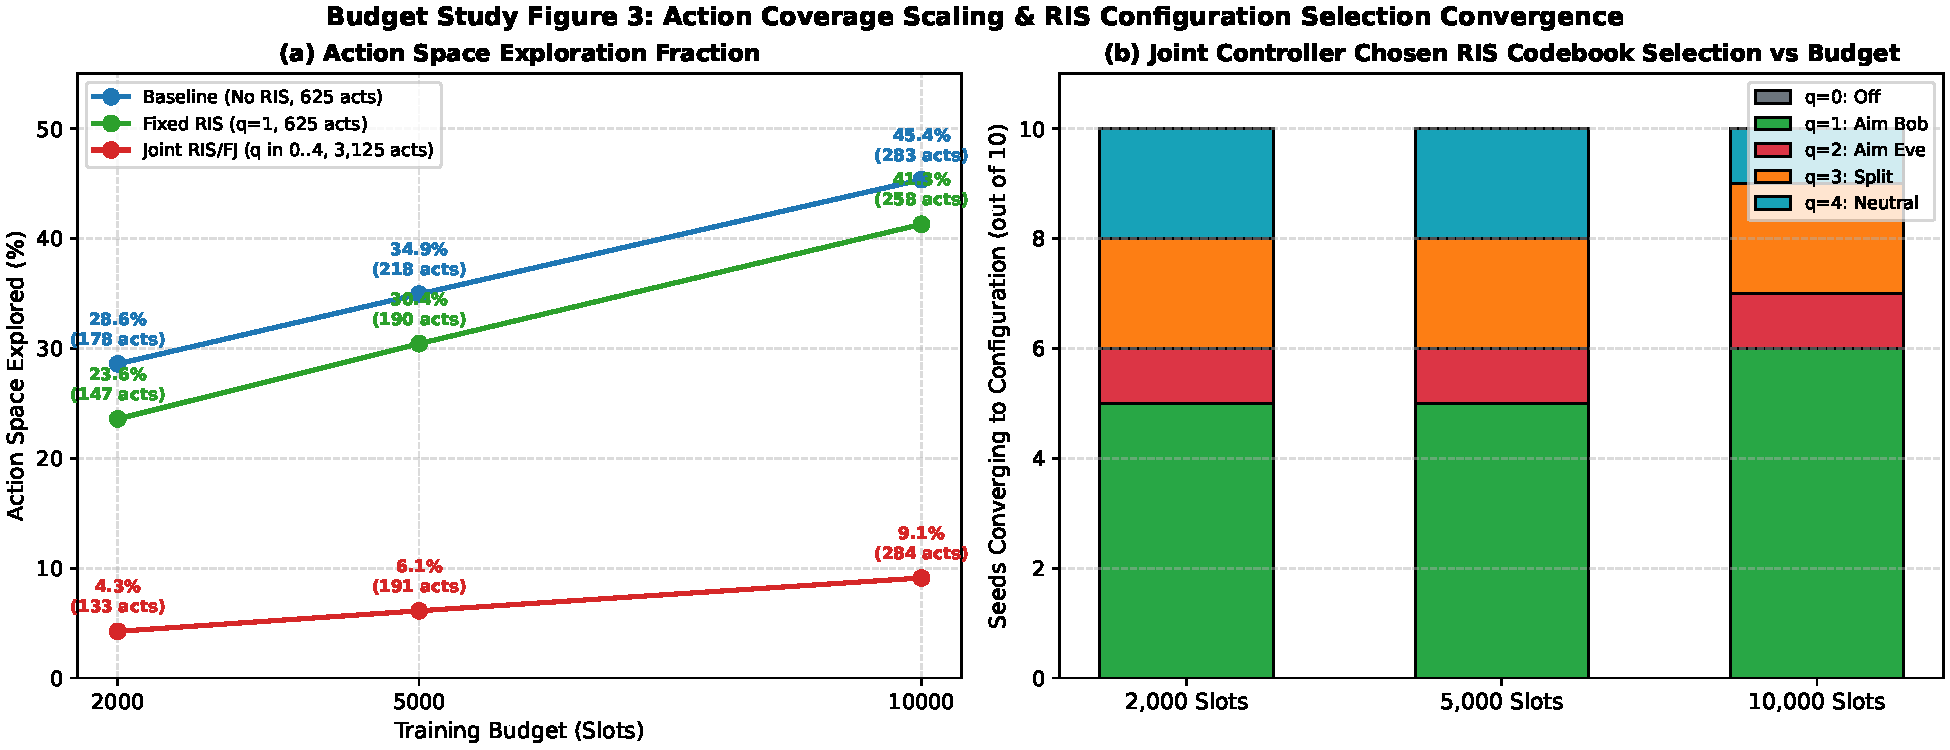
\includegraphics[width=\columnwidth]{figures/fig3_budget_coverage_and_q.pdf}
\caption{(a) Action space exploration percentage vs budget; (b) Converged RIS configuration selection distribution ($q \in \{0, 1, 2, 3, 4\}$) across 10 matched seeds.}
\label{fig:coverage}
\end{figure}

\begin{figure}[t]
\centering
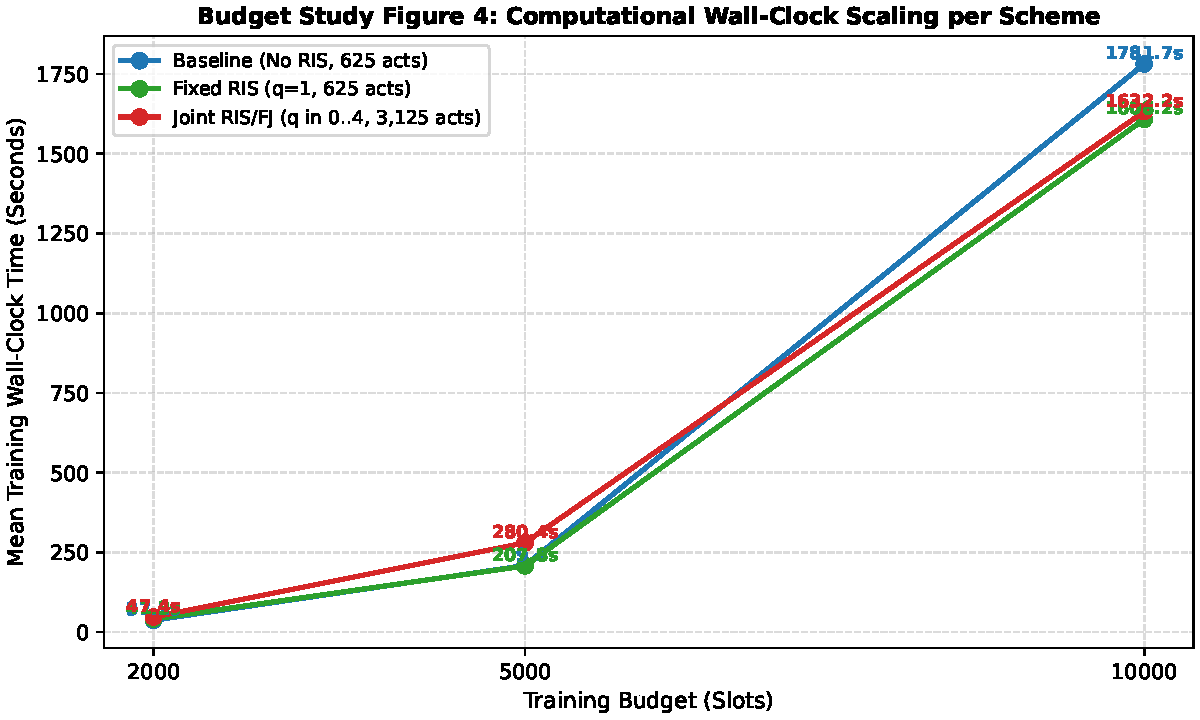
\includegraphics[width=0.85\columnwidth]{figures/fig4_computational_scaling.pdf}
\caption{Mean wall-clock training time per scheme across training budgets.}
\label{fig:scaling}
\end{figure}

\subsection{Primary Hypothesis Test: Joint vs. Fixed RIS}
As documented in Table II and Fig. \ref{fig:paired}, expanding the training budget to 10,000 slots yields a paired utility difference of:
\begin{equation}
\Delta U = +0.0183 \pm 0.0822, \quad 95\%\text{ CI } [-0.1677, +0.2043]
\end{equation}
with $t = +0.223$ and $p = 0.8289$. The null hypothesis cannot be rejected. Furthermore, Fixed RIS achieves a numerically higher secrecy rate ($1.5656$ vs. $1.4839$ bps/Hz, $\Delta R_s = -0.0817$ bps/Hz, $p = 0.4182$). 

\subsection{Mechanism: Action Space Dilution and Sub-Optimal Trapping}
Exhaustive finite-grid evaluation establishes that Configuration $q=1$ achieves the global maximum utility ($U^* = 0.9959$) and secrecy ($R_s^* = 1.8413$ bps/Hz) across all 3,125 actions. As shown in Fig. \ref{fig:coverage}(a), the Joint controller explores only $7.8\%$ (244 actions) of its action space at 10,000 slots due to the combinatorial 5-fold expansion. Consequently, Fig. \ref{fig:coverage}(b) reveals that 4 out of 10 seeds in Joint control remain permanently trapped in sub-optimal configurations ($q=2, 3, 4$), pulling group performance down.

\subsection{Decisive Advantage of Optical RIS Over Baseline}
At 10,000 slots, Fixed RIS achieves a decisive gain over the no-RIS baseline ($\Delta U = +0.2051 \pm 0.0367$, $t = +5.585$, $p = 0.00034$), demonstrating that passive specular optical RIS panels provide major security benefits in indoor VLC systems.

\section{Conclusion}
In this paper, we conducted a matched training-budget empirical study of optical RIS and friendly jamming control in secure visible light communication. By matching architectures ($m_0=11$, 497,000 parameters) across 90 complete runs, we established that expanding the training budget five-fold does not allow the Joint controller to statistically outperform Fixed RIS ($\Delta U = +0.0183$, $p = 0.8289$). Due to action-space dilution, the Joint controller leaves over $92\%$ of actions unexplored and frequently traps in sub-optimal RIS configurations. We conclude that in stationary indoor VLC environments, decoupling optical RIS alignment from dynamic friendly jamming optimization is physically and computationally superior to joint control.

\bibliographystyle{IEEEtran}
\bibliography{references}

\end{document}
